\documentclass[12pt]{article}
\usepackage{geometry}
\geometry{margin=1in}
\usepackage{xcolor}
\usepackage{soul}
\usepackage{forest}
\usepackage{hyperref}
\usepackage{graphicx}
\usepackage{float}
\title{Notes for An Introduction to Brain and Behavior}
\author{tzy}
\begin{document}
\maketitle
\tableofcontents
\newpage
\section{Basics}

\subsection{Vocabulary}

\begin{figure}[h]
    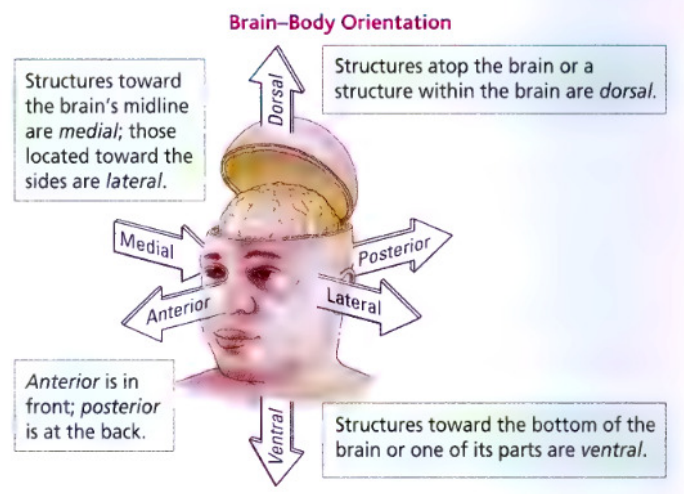
\includegraphics[width=0.88\textwidth]{brain_body_orientation.png}
\end{figure}

\textbf{Spatial Locations}
\begin{itemize}
\item {\textbf{Anterior}:   in the front}
\item {\textbf{Posterior}:  in the back}
\item {\textbf{Medial}:     to the middle}
\item {\textbf{Lateral}:    to the sides}
\item {\textbf{Dorsal}:     to the top}
\item {\textbf{Ventral}:    to the bottom}
\end{itemize}

\begin{figure}[H]
    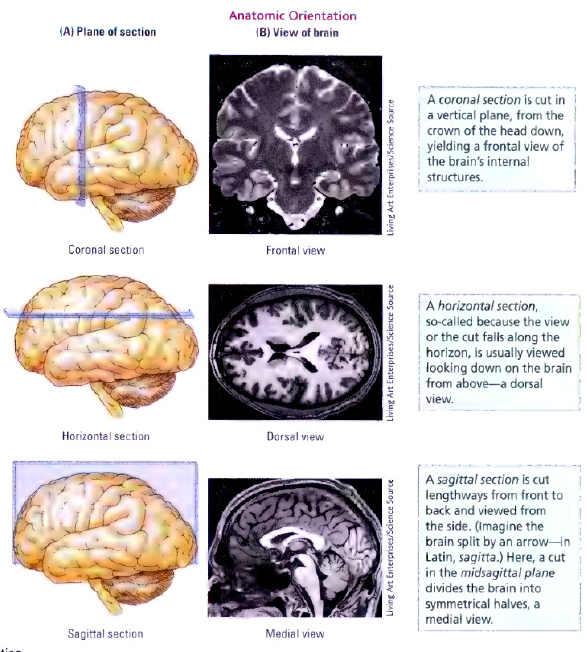
\includegraphics[width=\textwidth]{anatomical_orientation.png}
\end{figure}

\noindent \textbf{Anatomical Orientation}
illustrates the direction of a cut
\begin{itemize}
\item {\textbf{Coronal section}     \(\rightarrow\) frontal view}
\item {\textbf{Horizontal section}  \(\rightarrow\) dorsal view}
\item {\textbf{Sagittal section}    \(\rightarrow\) medial view}
\end{itemize}

\newpage
\section{Chapter 2}
\subsection{Plastic Patterns of Neural Organization}
Neural tissue has the capacity to change in response to the wold by changing how it is organized. Especially, \textbf{Learning} means changes in neural circuits.

This is called \textbf{neuralplasticity}, which is a part of \textbf{phenotypic plasticity}, which means that the same gene can express itself differently in respond to the environment.

e.g. People who suffer from cerebellar agenesis can slowly adapt; blind people can have enhanced auditory capacities. 


\subsection{Functional Organization of the Nervous System}

\begin{itemize}
\item {
    \textbf{The CNS}: 
    Brain and the spinal cord.
}\item {
    \textbf{The Somatic Nerves System (SNS)}: 
    Spinal and cranial nerves that carries incoming sensory information to CNS and transmit outgoing motor instructions from CNS.
}\item {
    \textbf{Autonomic Nerves System (ANS)}: 
    includes \textbf{parasympathetic nerves} that produces rest-and-digest response and \textbf{sympathetic nerves} that produces fight-or-flight response
}\item {
    \textbf{Enteric Nervous System (ENS)}: 
    A mesh of neurons embedded in the lining of gut, controls the gut. The ENS can communicate with the CNS via ANS but mostly operates autonomously}
\end{itemize}

\begin{figure}[H]
    \centering
    \footnotesize
    \begin{forest}
        for tree={
            align=center
        },
        [
            Nervous System
            [
                Central Nervous System (CNS)
                [
                    Brain
                ]
                [
                    Spinal cord
                ]
            ]
            [
                Peripheral Nervous System (PNS)
                [
                    Somatic\\Nervous System
                ]
                [
                    Autonomic\\Nervous System
                ]
                [
                    Enteric\\Nervous System
                ]
            ]
        ]
    \end{forest}
    \caption{Anatomical Organization}
\end{figure}


\begin{figure}[H]
    \centering
    \footnotesize
    \begin{forest}
        for tree={align=center},[
            Nervous System
            [
                Central\\
                Nervous System
                [
                    Brain
                ]
                [
                    Spinal cord
                ]
            ]
            [
                Somatic\\
                Nervous System
                [
                    Cranial\\
                    Nerves
                ]
                [
                    Spinal\\
                    Nerves
                ]
            ]
            [
                Autonomic\\
                Nervous System
                [
                    Sympathetic\\
                    Division (arousing)
                ]
                [
                    Parasympathetic\\
                    Division (calming)
                ]
            ]
            [
                Enteric\\
                Nervous System
            ]
        ]
        \end{forest}
    \caption{Functional Organization}
\end{figure}

\subsection{The Brain Surface Structure}
\begin{itemize}
\item {skull}
\item {
    meninges
    \begin{itemize}
    \item {Dura mater (from Latin, meaning ``hard mather'', which is a durable layer of fibrous tissue)}
    \item {Arachnoid membrane (from Greek, meaning ``spider's web'')}
    \item {Pia mater (from Latin, meaning ``soft mather'' which covers the brain)}
    \end{itemize}
}
\item {subarachnoid space (filled with cerebrospinal fluid (CSF), \hl{between} arachnoid layer and pia mater)}
\end{itemize}

\subsection{Cerebral Geography}

\begin{itemize}
\item {\textbf{Cerebral cortex}
    \begin{itemize}
    \item {\textbf{frontal lobe}: decision making, voluntary movement}
    \item {\textbf{parietal lobe}: motor functions}
    \item {\textbf{temporal lobe}: hearing, language, music, facial recognition and emotional processing}
    \item {\textbf{occipital lobe}: visual scene processing}
    \end{itemize}
}
\item {\textbf{Cerebellum}}
\item {\textbf{Brain stem}}
\end{itemize}
\begin{figure}[h]
    \centering
    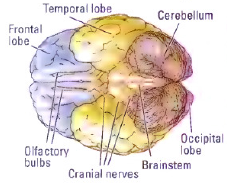
\includegraphics[width=0.55\textwidth]{ventral_view_brain.png}
    \caption{Ventral view of the brain}
\end{figure}

\subsection{Cerebral Circulation}

\end{document}